% we pad zero to the 2D image features by the largest kernel size. And we transform the kernel to match the padded image feature. To compute convolution, we compute element-wise product with the transformed kernel and sum all the features. Unlike \cite{Podlozhnyuk}, we do not need to shift the data nor kernel if we use simple mathematical trick. 
%   
% \begin{align}
%     x_{pad} & = \mathcal{P}_{n+m}(x)\\
%     y_{pad} & = \mathcal{P}_{n+m}(y)\\
%     x_{pad} \ast y_{pad} & = \mathcal{F}^{-1}(\mathcal{F}(x_{pad}) \circ \mathcal{F}(y_{pad}))
% \end{align}
% 
%   Where $\ast$ is the circular convolution and $\circ$ is the Hadamard Product and $\mathcal{F}$ is the Fourier Transformation and $\mathcal{P}_n$ is the padding operation that append zeros to make vector of size $n$.
% 
% For each dimension of features, we transform kernel and image feature into frequency domain using Fast Fourier Transformation. We transform the image into frequency domain once and use the transformed image for all templates.
% 
% We implemented the convolution using FFT on GPU and got 10x speed up.


% \subsubsection{Fast Convolution using the FFT}

% We compare the performance of WHO and NZ-WHO on 3D Object dataset \cite{Savarese07} and report performance on Table \ref{tab:who_initializations}. 

% To deal with the problems, we propose Non-Zero Whitened Histograms of Orientations.

% To accommodate the growing usage of rendering image for 2D-3D matching using
% WHO\cite{Aubry13, Aubry14, Lim14}, we analyzed various methods to whiten
% synthetic rendering image and propose Non-Zero Whitened Histograms of
% Orientations (NZ-WHO) which is a direct extension of \cite{Hariharan12}
% designed for rendering images with textureless background. % Since a NZ-WHO
% template has zero-mean and all elements in the template follow same
% distribution, no explicit calibration is required if all the templates have
% approximately the same number of cells. 

% Since Combining NZ-WHO with Conjugate Gradient, 

% \subsection{Non-Zero Whitened Histograms of Orientations (NZ-WHO)}
% why non zero whitening and why it makes more sense than seeing 3D, IKEA
% Overview of the subsections
%   Generating covariance quickly
%   Fast inversion
%   Regularization
% Overview of the subsections
% In this section, we will give a brief overview of whole whitening stages. In the first section \ref{feature_statistics}, we will discuss about first and second order statistics of HOG feature. Then, we will discuss about using autocovariance $\Gamma$ to create covariance matrix $\Sigma$ for non-zero cells and SIMD implementation to speed up the generation. Then, we will explain fast and accurate way to solve $w = \Sigma^{-1}x$ using Conjugate Gradient method. % Finally, we will analyze the effect of regularization.

% \subsection{Whitening and Textureless Background}
\begin{comment}
\subsection{Constructing the Covariance Matrix}
\label{sec:feature_statistics}
% Whats used in our work and using Autocovariance matrix
We first collected the first and second order statistics (mean and
autocovariance) of HOG features from arbitrary natural images. Following
\cite{Hariharan12}, we assume Wide-Sense Stationarity (WSS) of HOG features
generated from natural images. That is, we assume the mean of a HOG cell is
independent of its place in the image, and the autocovariance of patches depends
only on their relative location.

In one dimension, let $x(u)$ be the feature at location $u$. Then WSS states
that $\mathbb{E}\left[x(u)\right] = \mu_x$ for all $u$, and
\begin{equation}
\textrm{cov}_x(u,v) = \textrm{cov}_x(0, v-u) = \Gamma(v-u),
\end{equation} where $\Gamma$ is the autocovariance. For simplicity, we show the 1D case but this can be easily extended to 2D spatial autocovariance.

Therefore, assuming WSS allows us to synthesize the covariance matrix for
templates \emph{of any size} from the autocovariance matrix. This hugely reduces
the memory required because to build the covariance matrix of a template of $w
\times h$ HOG cells (with 31 elements per cell), we only need a $w \times h
\times 31$ autocovariance matrix. In comparison, the covariance matrix itself is
$(w \times h \times 31) \times (w \times h \times 31)$. Furthermore, by using
the autocovariance we can avoid storing the covariance matrix for every
different aspect ratio used during detection.

To further simplify $\Gamma$, we assumed horizontal and vertical symmetry. In
our implementation, we compute a $40 \times 40 \times 31$ autocovariance matrix,
meaning we can synthesize covariance matrices for HOG grids as big as $40 \times
40$. In practice we limit the number of cells per template to 250.

We use the GPU to parallelize the lookup of the correct autocovariance cells
during covariance matrix syntheses. The real time analysis for various number of cells is on Figure \ref{fig:covariancetime}).

\end{comment}

% Since the statistics have been computed for a generic HOG feature, we can use
% the same statistics for all templates and images. In practice, since it is
% expensive to whiten all the sliding patches in the image, we followed
% \cite{Hariharan12} and defined the templates to be $w =
% \Sigma^{-1}(X-E[X])$\begin{comment}which is a good approximation of
% $\Sigma^{-\frac{T}{2}} \Sigma^{-\frac{1}{2}}(X-E[X])$\end{comment} 

% \begin{comment}Gathering statistics, especially computing spatial covariance
% of a signal is computationally burdensome. \end{comment} To speed up the
% statistics collection, \begin{comment}in addition to the wide-sense
% stationarity (WSS) of HOG, \end{comment}we assumed horizontal and vertical
% symmetry of covariance. 

 %Hariharan \etal \cite{Hariharan12} interpreted the whitening also as the
 %Linear Discriminant Analysis where each class has the same covariance $\Sigma$
 %but with different mean value. They defined this whitened HOG feature as
 %Whitened Histograms of Orientations (WHO) and we will follow their convention
 %of the name.

% \subsection{Rendering}
% 
% We used a public rendering engine to create realistic rendering and
% depth\begin{comment}\cite{Choy14render}\end{comment}. The CAD models we used
% in our experiments contain color, texture and material information such as
% transparency and reflectance. We tried to make the rendering as much realistic
% as possible to simulate the natural image statistics. The example rendering is
% in Fig. \ref{fig:rendering}. We also extracted depth information as well while
% rendering to use in the reconstruction.


% To whiten a HOG features, we first have to synthesize the covariance matrix.
% Following the method of \cite{Hariharan12}, which assumes spatial Wide-Sense
% Stationarity (WSS) of a feature, covariance matrix can be synthesized using
% spatial autocovariance $\Gamma$. This assumes the \begin{comment} and features
% such as HOG are gradients in a small patch whose statistics does not change
% (an object can be in anywhere in an image)\end{comment}. 

%However, unlike small fixed-sized mid-level patches, the root templates have
%different aspect ratios, different gradient patterns and large number of HOG
%cells which results in large covariance $\Sigma \in \mathcal{R}^{7000 \times
%7000}$ that is difficult to cache. Thus, to generate a NZ-WHO template, we have
%to synthesize a covariance matrix and solve the system of linear equations. 



% Thus, every time we whiten a root template, we have to generate a covariance
% matrix using autocovariance $\Gamma$. 

%\begin{comment} Also, since we are whitening only the non-zero HOG cells whose
%position is unknown beforehand and all templates have different aspect ratio
%for , we cannot cache the matrix. Using CPU, it takes about \end{comment}

% In practice, synthesizing covariance matrix $\Sigma$ takes long time due to
% its large size.  $\Sigma$ ranges from $\Sigma \in \mathcal{R}^{7000 \times
% 7000}$ to $\Sigma \in \mathcal{R}^{7500 \times 7500}$. We vary the template
% resolution and run $\Sigma$ generation on CPU and GPU 100 times and report the
% average time in Fig. \ref{fig:covariancetime}.

% \begin{figure}[t]
%   \begin{center}
%      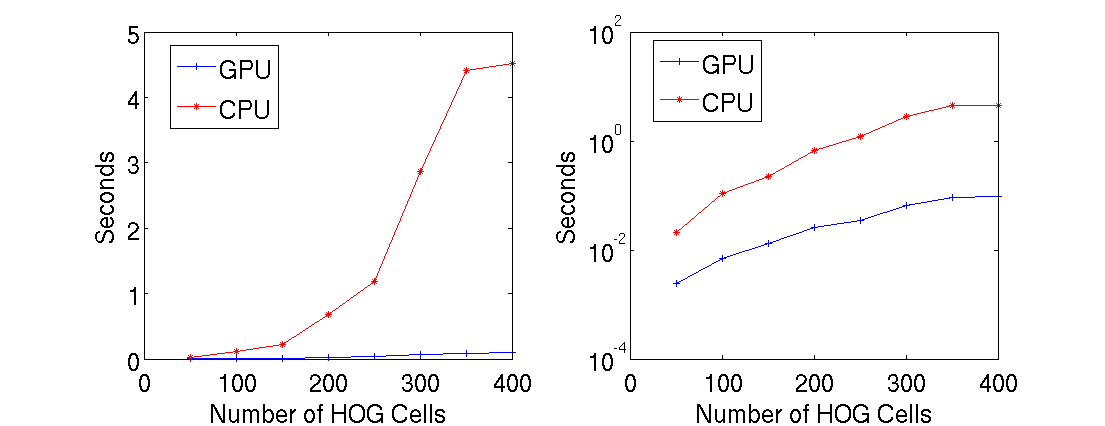
\includegraphics[width=0.9\linewidth]{covariancetime} 
%   \end{center}
%   \caption{Time to generate $\Sigma$ for various number of cells (left) and same plot on log scale(right). The time complexity increases as $O(n^2)$ for $n$ number of cells.}
%   \label{fig:covariancetime_crop}
% \end{figure}
 
% 1-dimensional version of SIMD implementation that generate covariance matrix $\Sigma$ from autocovariance $\Gamma$ on GPU is on the supplementary material.
% \begin{comment}i
% \begin{algorithm}
% \KwData{ $\Gamma$ , nonzero cell indexes, thread x id, thread y id}
% \KwResult{ $\Sigma$ }
% \Begin{
% $c_u \leftarrow \mod(x, N_f)$ define cell $u$ coordinate\; 
% $f_u \leftarrow u / N_f$ define feature index
% $c_v \leftarrow \mod(y, N_f)$ define cell $v$ coordinate\;
% $f_v \leftarrow v / N_f$ define feature index
% $T \leftarrow $ nonzero cell indexes\;
% $\Sigma(w) \leftarrow \Gamma( N_f ( T(u) - T(v) +  )$\;
% }
% \caption{SIMD implementation of covariance synthesis from autocovariance}
% \end{algorithm}
% \end{comment}



% The final challenge in on-the-fly template evaluation is performing the
% convolution between the template and the target image. Standard convolution
% would be prohibitively slow for the high resolution templates we're using, so we
% implemented the convolution via Fast Fourier Transform on the GPU. This allows
% template evaluation to run in \scream{x ms}, compared to \scream{x ms} for the
% naive CPU implementation.

  
%  If we use a high resolution template such as \ref{fig:rendering}

% where $w$ is the weight we want to find and $x$ is the HOG feature from the
% rendering and $\lambda$ is the regularization constant (see section
% \ref{sec:regularization}). For $w\in \mathcal{R}^n$, it takes $O(n^3)$ time to
% solve the linear equation. If we use a high resolution template to capture
% small geometric properties we can get high accuracy matchings but the solving
% the linear equation becomes computationally burdensome. 

% To briefly recap, the LU Decomposition and Cholesky Decomposition are most
% popular methods to solve a linear equation. In linear algebra libraries such
% as MATLAB, these decomposition methods are default method to solve a linear
% equation (backslash \textbackslash in MATLAB). Since the covariance matrix is
% Hermitian and Positive Semi-Definite, we can use Cholesky Decomposition which
% is twice as fast as the LU Decomposition.  

% decomposition methods such as LU or Cholesky Decomposition not only take long
% time but they also accumulate numerical error. 

%In our setting, we used high resolution template which has more than 250 HOG
%cells. This result in $\Sigma \in \mathcal{R}^{7500 \times 7500}$. It takes
%about 9 seconds if we use LU decomposition and 5 seconds if we use Cholesky
%decomposition.  % The default way of solving the linear equation in many linear
%algebra library is decomposing the matrix using LU Decomposition (in MATLAB the
%default method of backslash operator) which takes $O(\frac{2}{3}n^3)$ flops for
%$n\times n$ matrix. Since the matrix, $\Sigma + \lambda I$ is Hermitian and
%Positive Semi Definite. We can speed up using Cholesky Decomposition. 



%We also used iterative Conjugate Gradient to make use of low rank property of
%the covariance \cite{Gharbi12}. After adding small regularization, the
%regularized covariance matrix has nice spectral property (Figure
%\ref{fig:spectral}). The singular values are clustered in small region and most
%of the energies are concentrated on the first (number) singular values. Thus,
%the conjugate gradients stage doesn't go upto the size of the matrix to
%converge.

[Figure spectral analysis]

\subsection{Variations of WHO}
\scream{sam thinks this should be moved to the experiments section}
We empirically found out that NZ-WHO performs reasonably well without time
consuming calibration stage compare to other variational method to generate
templates. We used 1 CAD model with viewpoints covering 24 azimuths and 4
elevations. Each template takes approximately 80 milliseconds to generate a
NZ-WHO template. We also calibrated templates using the method presented in
\cite{Aubry14}. The calibration learns affine transformation of the detection
confidence.% Note that in Section \ref{experiments}, we provide the same
experiment with 9 CAD models.


\begin{table*}[!htbp]
    \footnotesize
    \begin{center}
\begin{tabular}{|c|c|r|c|r|}
\hline
Methods (AP/MPPE) & before calibration  & time & after calibration \cite{Aubry14} & time \\
\hline\hline
HOG\cite{Dalal05}     & 72.3 / 65.0           &  31ms  & 60.4 / 50.2                 & 8.7 sec \\ 
WHO\cite{Hariharan12} & 82.1 / 85.4           &  3811ms& 84.4 / 83.0                 & 12.4 sec  \\
WHO-CG                & 81.7 / \textbf{84.9}  &  104ms & 83.7 / 87.3                 & 8.3 sec \\
WHO-CG-Z              & 54.4 / 65.1           &  103ms & \textbf{92.8} / 86.7        & 8.7 sec  \\
% NZC-WHO-Z    & 89.10/\textbf{78.64} &    & 91.15/74.79                  &     \\
NZ-WHO-CG             & \textbf{90.0} / 82.8  &   79ms & 90.3 / \textbf{86.8}        & 8.5 sec   \\
\hline
\end{tabular}
\end{center}
\caption{Average Precision(AP) and Mean Precision in Pose Estimation (MPPE) \cite{Lopez-Sastre11} variations of WHO on 3DObject Car dataset\cite{Savarese07}. WHO refers to standard WHO using the method presented in \cite{Hariharan12}, WHO-CG uses iterative Conjugate Gradient method to generate WHO. WHO-CG-Z uses whiten the whole template and zero out textureless region. NZ-WHO-CG is the NZ-WHO which whitens only non-zero cells using iterative Conjugate Gradient method. The time column indicates the time to generate one template. We followed calibration procedure presented in \cite{Aubry14}.}
\label{tab:who_initializations}
\end{table*}

We found out that without calibration, NZ-WHO performs the best on object
detection on 3DObject car dataset \cite{Savarese07}. See Table
\ref{tab:who_initializations} for detail. In essence, if we use calibration, we
could achieve better performance but since our goal is to do 2D-3D matching and
continuous viewpoint estimation using on-the-fly template generation, we did not
calibrated our templates.


\begin{comment}
\subsection{Whitening Non-Zero Cells}

% learning weights for whitened templates
But since it is difficult to make templates to have the number of cells, \cite{Hariharan12, Aubry14, Lim14} learned weights for convolution score from the template. However, we propose a novel way to guarantee normalized score distribution by decorrelating non-zero HOG cells and forcing each template to have approximately same number of cells.

% 
Unlike \cite{Aubry14}, we did not whiten all cells and then zero out some HOG cells that are on the background. Instead, we whiten only the cells with non-zero value. We empirically found out that by whitening the cells that has non-zero support actually performs better and takes less time solving the linear equation $w = \Sigma^{-1}x$ since the number of elements to whiten decreases. However, by selecting non-zero cells, we destroys inherent Toeplitz-Block-Toeplitz property of the covariance matrix which could speed up the inversion using Fourier Transformation \cite{Akaike73, Martinsson05}.

  We propose a whitening stage for WHO feature template generation that can create template whose convolution score follow same distribution. This guarantees that we do not require any calibration stage after generating templates rapidly. We statistically compare the score distribution of whitening non-zero HOG cell only and whitening.
  \end{comment}


% \subsection{Effect of Regularization}
% \label{sec:regularization}
%  Also, since all covariance matrix is Positive Semi Definite, our matrix
%  $\Sigma$ must be Positive Semi-Definite too. To guarantee the property, We
%  found out that the regularization has significant impact on the performance.
%  In \cite{Hariharan12}, Hariharan \etal used small fixed regularization since
%  the covariance matrix of specially correlated features is intrinsically
%  row-rank to make the matrix invertible.
%  
% However if we closely analyze the impact of the regularization, we can see that larger the $\lambda$ is, the centered HOG becomes more dominant. 
% 
% \begin{align}
% (\Sigma + \lambda I)^{-1} & = \frac{1}{\lambda}\left(I + \frac{1}{\lambda}\Sigma \right)^{-1} \\
% & = \frac{1}{\lambda}\left(I - \frac{1}{\lambda} \Sigma  + \frac{1}{\lambda^2} \Sigma^{2} 
% 		- \frac{1}{\lambda^3} \Sigma^{3} + \cdots \right)
% % & = \frac{1}{\lambda}I - \left(I + \frac{1}{\lambda} \Sigma \right)^{-1} \frac{1}{\lambda^2} \Sigma
% % & = \frac{1}{\lambda}\left(I  - \frac{1}{1 + \frac{1}{\Sigma} \Tr{\Sigma}} \right)
% \end{align} 
% 
% We empirically found out that as $\lambda$ increases, AP converges to that of centered HOG feature without any whitening.

\begin{comment}
\subsection{No Calibration}
  We created coarse viewpoint templates by whitening non-zero HOG cells and compare the average precision on 3D Object dataset \cite{Savarese07} with that of whitening all HOG cells. 
  
\begin{table}
\begin{center}
\begin{tabular}{|l|c|c|}
\hline
Whitening and AP & Whiten & No Whitening \\
\hline\hline
Average Precision & 89.205 & 74.478 \\
\hline
\end{tabular}
\end{center}
\caption{Effect of whitening on 3D Object Car validation set using one CAD model. The whitening dramatically increased the AP.}
\end{table}
\begin{table}
\begin{center}
\begin{tabular}{|l|c|c|}
\hline
Calibration methods \&AP & Whiten non-zero & Whiten all \\
\hline\hline
None & 89.205 & 86.676 \\
Linear & 88.430 & 85.720 \\
Gaussian & 87.913 & 84.567\\
Number of non-zero cells & 84.734 & N/A\\
\hline
\end{tabular}
\end{center}
\caption{Various calibration and AP on small experimental set. Since the whitening templates with constant number of HOG cells create normalized feature, calibration using negative patches did not improve the AP.}
\end{table}
\end{comment}

%------------------------------------------------------------------------


